\documentclass[a4paper, 12pt]{report}

\usepackage[italian]{babel}
\usepackage{graphicx}
\usepackage{float}
\usepackage{tabularx}
\usepackage{ltablex}
\usepackage[font=small,format=plain,labelfont=bf,up,textfont=normal,up,justification=justified,singlelinecheck=false,skip=0.01\linewidth]{caption}
\renewcommand{\familydefault}{\sfdefault}

\title{"Progetto di una base di dati per la gestione del ciclo di vita del difetto nella produzione dell'elettrodomestico"}
\author{Castellucci Matteo\\Matricola 0000825436\\Anno accademico 2018-2019}
\date{\today}

\begin{document}

\maketitle

\tableofcontents

\chapter{Introduzione}
In questo progetto si vuole realizzare una base di dati a supporto della gestione dei difetti nella realizzazione dell'elettrodomestico,
chiudendo la "catena dell'informazione" tra cliente ed azienda nella fase terminale del ciclo di vita del prodotto. Lo scopo è fornire
all'azienda tutte le informazioni necessarie sugli elettrodomestici una volta arrivati nelle mani del cliente finale, così da poter
ottenere informazioni sul campo per quanto riguarda gli obiettivi attesi e disattesi. In particolar modo, l'attenzione è posta sull'elemento
principe per quanto rigurda l'analisi del comportamento di un bene di consumo: il difetto, in tutti i suoi aspetti. Sarà permesso a tutti gli
attori in gioco, tecnici, telefonisti, analisti dei dati e progettisti, di poter avere una visione a tutto tondo del problema che riguarda
il prodotto: le tempistiche di manifestazione, di risoluzione, il tipo di guasto ed altro ancora. Questo permetterà all'azienda di poter
avere più controllo sullo sviluppo e la messa in produzione di futuri progetti avendo a disposizione più informazioni strategiche.

\chapter{Analisi}

\section{Intervista}
Si vuole realizzare una base di dati che permetta di gestire tutte le informazioni che riguardano un guasto di un elettrodomestico.
L'azienda riceve telefonate da un cliente che vengono smistate ad un adeguato centro assistenza dove ciascuna verrà raccolta da un operatore.
Ogni centro assistenza ha sede in una città e possiede una determinata area di competenza, per cui tutte le chiamate che verranno effettuate
all'interno di quest'ultima verranno redirette al centro assistenza associato. L'identificazione dei centri assistenza viene fatta mediante dei
codici che hanno però valenza solamente nazionale.\newline
L'operatore, di cui l'azienda conosce dati identificativi come nome, cognome, data e luogo di nascita, codice fiscale, luogo di residenza, nonchè lo 
stipendio che gli elargisce, così come per ogni suo dipendente, chiede al cliente di identificarsi. Vengono richiesti dall'operatore 
il nome, il cognome e il recapito a cui fare riferimento nel momento nel quale un solo tecnico si recherà in loco per riparare il suo elettrodomestico. 
Eventualmente, l'operatore chiede anche l'indirizzo \textit{email}, qualora il cliente lo possieda. Inoltre, viene registrato il numero di telefono 
chiamante a cui verrà fatto riferimento anche in futuro come specifico per quel dato cliente.\newline
In seguito, l'operatore chiede quale prodotto o quali prodotti del cliente hanno subito un guasto e saranno l'oggetto della corrente richiesta di 
assistenza. L'operatore per ogni elettrodomestico ne chiede la categoria, il modello, specificato con un codice, e si fa leggere "PNC" (\textit{Product 
Number Code}), che lo identifica univocamente trattenendo informazioni sulla sua produzione e "SNC" (\textit{Serial Number Code}), che specifica ulteriori 
informazioni tecniche. L'operatore richiede inoltre la data di acquisto dell'elettrodomestico e la data di installazione dello stesso e le registra qualora 
il cliente le abbia a disposizione o se ne ricordi. In assenza di data di acquisto sarà compito del tecnico, una volta recatosi a casa del cliente, 
recuperare almeno questa informazione e in caso la garanzia del prodotto sia scaduta o non sia trovata, far pagare il cliente. Il cliente potrebbe avere 
aderito opzionalmente ad un programma di estensione della garanzia, identificato da un codice, informazione che deve fornire, se non fase in chiamata, 
almeno al momento della visita. Da ultimo, l'operatore chiede al cliente di farsi descrivere il guasto e registra la data corrente come data di apertura 
della pratica, ponendo lo stato dell'intervento come aperto e concorda con il cliente la data di visita del tecnico a casa per la riparazione.\newline
Un difetto è univocamente determinato da due codici, il "\textit{Component Code}", che identifica quale parte di un elettrodomestico viene affetto, e
il codice di tipo, che indica qual è nello specifico il tipo di difetto che il componente può subire. Ad ogni difetto sono associati i ricambi che sono 
necessari per poterlo sistemare, che potrebbero anche essere più di uno o nessuno, identificati da un codice, e il costo di ciascuno di essi, 
sia in termini di costo del ricambio stesso, che del costo di manodopera per l'installazione.\newline
Un tecnico, che afferisce ad un centro assistenza come l'operatore, si preoccuperà, una volta raccolte le informazioni necessarie dalla chiamata,
di recarsi a casa del cliente e registrare a sua volta una descrizione personale del guasto del cliente, dopodichè possibilmente riparerà il guasto
e si preoccuperà di chiudere la richiesta di assistenza pendente. Specificherà anche il tempo che ha impiegato nel risolvere il problema del cliente
espresso in quarti d'ora. Un tecnico può lavorare direttamente per l'azienda o è assunto tramite un'impresa terza per l'azienda stessa. \newline
Un progettista di elettrodomestici dovrà poi periodicamente recuperare le informazioni riguardanti i guasti che si sono verificati sui prodotti che
gli competono, indicati dalla o dalle categorie di prodotto a cui è assegnato, e stilare rapporti che possano aiutare l'azienda a migliorare la produzione.

\section{Analisi ed eliminazione delle ambiguità}

\begin{tabularx}{\linewidth}{X|X}
	\hline
	\textbf{Termine presente nel testo} & \textbf{Sinonimo utilizzato}\\
	\hline
	\hline
	Elettrodomestico & Prodotto\\
	\hline
	Pratica & Intervento\\
	\hline
	Telefonata & Intervento\\
	\hline
	Richiesta di assistenza & Intervento\\
	\hline
	Chiamata & Intervento\\
	\hline
	Riparazione & Intervento\\
	\hline
	\caption{Associazioni termine-sinonimo per formulare specifiche non ambigue}
\end{tabularx}

Il termine "elettrodomestico" verrà da qui in avanti sostituito dal termine "prodotto", in quanto dotato di una più adeguato carattere di astrattezza
e generalità, benchè il caso in esame sia studiato su di un'azienda che produce elettrodomestici. I termini come "chiamata", "richiesta di
assistenza", "intervento" e loro sinonimi vengono tutti raccolti sotto il termine "intervento" poichè di fatto descrivono le varie fasi dello
stesso, dalla richiesta iniziale del cliente, alla visita del tecnico dell'assistenza, fino alla riparazione del prodotto indicato. Si intende
che ogni intervento sarà raccolto in un'unica pratica e perciò anche quest'ultimo termine indica lo stesso concetto.

\section{Definizione delle specifiche ed estrapolazione dei concetti}
Si vuole realizzare una base di dati che permetta di gestire tutte le informazioni che riguardano un  \textbf{guasto} di un \textbf{prodotto}.
Un prodotto è univocamente identificato da un "PNC" (\textit{Product Number Code}) ed è caratterizzato da una categoria, un \textbf{modello} 
sotto forma di codice e un "SNC" (\textit{Serial Number Code}). Un prodotto possiede inoltre una data di acquisto e una di installazione, insieme ad 
un'estensione di garanzia associata identificata da un codice, informazioni che però possono essere disponibili o meno, a seconda che il \textbf{cliente}
ne abbia tenuto traccia o meno.\newline
Al verificarsi di un guasto, il cliente si preoccupa di chiamare l'assistenza clienti dell'azienda produttrice per richiedere un
\textbf{intervento}. Ogni cliente verrà identificato dal suo numero di telefono e verranno registrati il suo nome, il suo cognome,
il recapito presso il quale dispacciare il \textbf{tecnico} per la riparazione del prodotto ed opzionalmente il suo indirizzo \textit{email},
solamente nel caso il cliente lo possedesse.\newline
Il cliente parlerà con un \textbf{operatore}, che chiederà al cliente tutte le informazioni relative al prodotto o ai prodotti
che hanno subito un guasto insieme ad una descrizione di quest'ultimo che viene anch'essa registrata. Viene inoltre concordata una data di
visita del tecnico affinchè possa riparare il prodotto. Infine, vengono registrati la data della chiamata del cliente e viene
aggiornato lo stato dell'intervento come aperto. Quando il tecnico visiterà il cliente, uno solo per intervento, registrerà una sua descrizione
del guasto e dopo averlo riparato segnerà lo stato dell'intervento come chiuso. Indicherà anche il tempo speso per farlo in quarti d'ora.\newline
Un guasto è associato ad uno specifico \textbf{difetto}, il quale è univocamente determinato da due codici: il "\textit{Component Code}"
che identifica il componente del prodotto coinvolto e un codice che identifica il tipo del difetto su quello specifico componente. Nella
riparazione di un difetto possono essere utilizzati uno o più \textbf{ricambi}, ognuno dei quali è identificato da un codice e vi è associato
sia un costo di acquisto per il ricambio stesso che di manodopera per l'installazione.\newline
L'azienda possiede per i suoi dipendenti informazioni come il codice fiscale, il nome, il cognome, la data e il luogo di nascita, luogo di
residenza e lo stipendio percepito. I dipendenti presi in considerazione sono gli operatori, i tecnici e i
\textbf{progettisti} di elettrodomestici. Gli operatori e i tecnici afferiscono ad uno specifico \textbf{centro assistenza} dell'azienda,
mentre i progettisti sono interessati ad analizzare i dati di una o più \textbf{categorie} di prodotto. Un tecnico inoltre può essere
dipendente interno dell'azienda oppure no.\newline
Un centro assistenza ha sede in una città e possiede una determinata area di competenza, nella quale tutte le telefonate che vengono fatte
per l'assistenza vengono inoltrate a quello specifico centro. Esso è identificato da un codice univoco, ma solo nella nazione in cui si trova.\newline

\begin{tabularx}{\linewidth}{>{\hsize=0.375\hsize}X|X|>{\hsize=0.475\hsize}X}
	\hline
	\textbf{Termine} & \textbf{Descrizione} & \textbf{Collegamenti}\\
	\hline
	\hline
	Prodotto & Un elettrodomestico che l'azienda ha rilasciato sul mercato ed è stato comprato da un cliente, per poi subire un guasto &
	Cliente,\newline
	Modello,\newline
	Guasto\\
	\hline
	Modello & Una classe di prodotti accomunata da caratteristiche comuni & Prodotto\\
	\hline
	Cliente & Una persona che ha acquistato un prodotto presso l'azienda e ha richiesto un intervento per quello specifico prodotto & Prodotto,\newline 
	Intervento\\
	\hline
	Guasto & Un problema di varia natura che si è verificato in uno specifico prodotto, causato da un difetto nel prodotto stesso & Prodotto,\newline 
	Difetto\\
	\hline
	Intervento & Una richiesta fatta da un cliente per risolvere un guasto subito, sarà registrato da un operatore, risolto da un tecnico ed
	analizzato da un progettista & Guasto,\newline Operatore,\newline Tecnico,\newline Progettista\\
	\hline
	Difetto & Una classe di guasti accomunati dal componente in cui il guasto si verifica e la natura del difetto stesso, possono essere utilizzati
	dei ricambi per poterlo riparare & Guasto,\newline Ricambio\\
	\hline
	Ricambio & Un componente di un prodotto che può essere utilizzato nella riparazione di un difetto & Prodotto,\newline Difetto\\
	\hline
	Operatore & Un dipendente dell'azienda che si preoccupa di aprire richieste di intervento, appartiene ad un determinato centro assistenza
	& Intervento,\newline Centro Assistenza\\
	\hline
	Tecnico & Un dipendente dell'azienda che si preoccupa di attendere ad interventi di manutenzione e chiudere le richieste pendenti, appartiene
	ad un centro assistenza & Intervento,\newline Centro Assistenza\\
	\hline
	Progettista & Un dipendente dell'azienda che si preoccupa di analizzare i dati sugli interventi effettuati, si occupa solamente di alcuni tipi
	di prodotto & Intervento\\
	\hline
	Centro Assistenza & Parte dell'azienda volta all'impiego di operatori e tecnici di assistenza & Operatore,\newline Tecnico\\
	\hline
	\caption{Glossario dei termini}
\end{tabularx}

\chapter{Analisi concettuale}

\section{Schema scheletro}

\begin{figure}[H]
	\centering
	%\includegraphics[width=\linewidth]{images/scheletro.png}
	\caption{Schema scheletro dei concetti, così come estrapolati dalle specifiche}
\end{figure}

\section{Raffinamenti proposti}

\subsection{Gerarchia di persone}

Nelle specifiche sono specificati quattro concetti - "cliente", "operatore", "tecnico" e "progettista" - che si prestano a diventare entità, ma
che ruotano tutte attorno alla nozione di persona. Tutte queste infatti sono persone e in quanto tali condividono almeno informazioni come il nome
ed il cognome; è perciò significativo metterle assieme in una gerarchia che discende da persona. Inoltre, tutti e tre i concetti meno che "cliente"
sono di fatto dipendenti dell'azienda e in quanto tali le informazioni che l'azienda trattiene su di essi sono le stesse, pur intrattenendo con gli
altri concetti rapporti diversi a seconda della mansione che svolgono. Anche per queste tre concetti è opportuno raccoglierli attraverso una seconda
gerarchia che origini da dipendente, che a sua volta è una persona.

\begin{figure}[H]
	\centering
	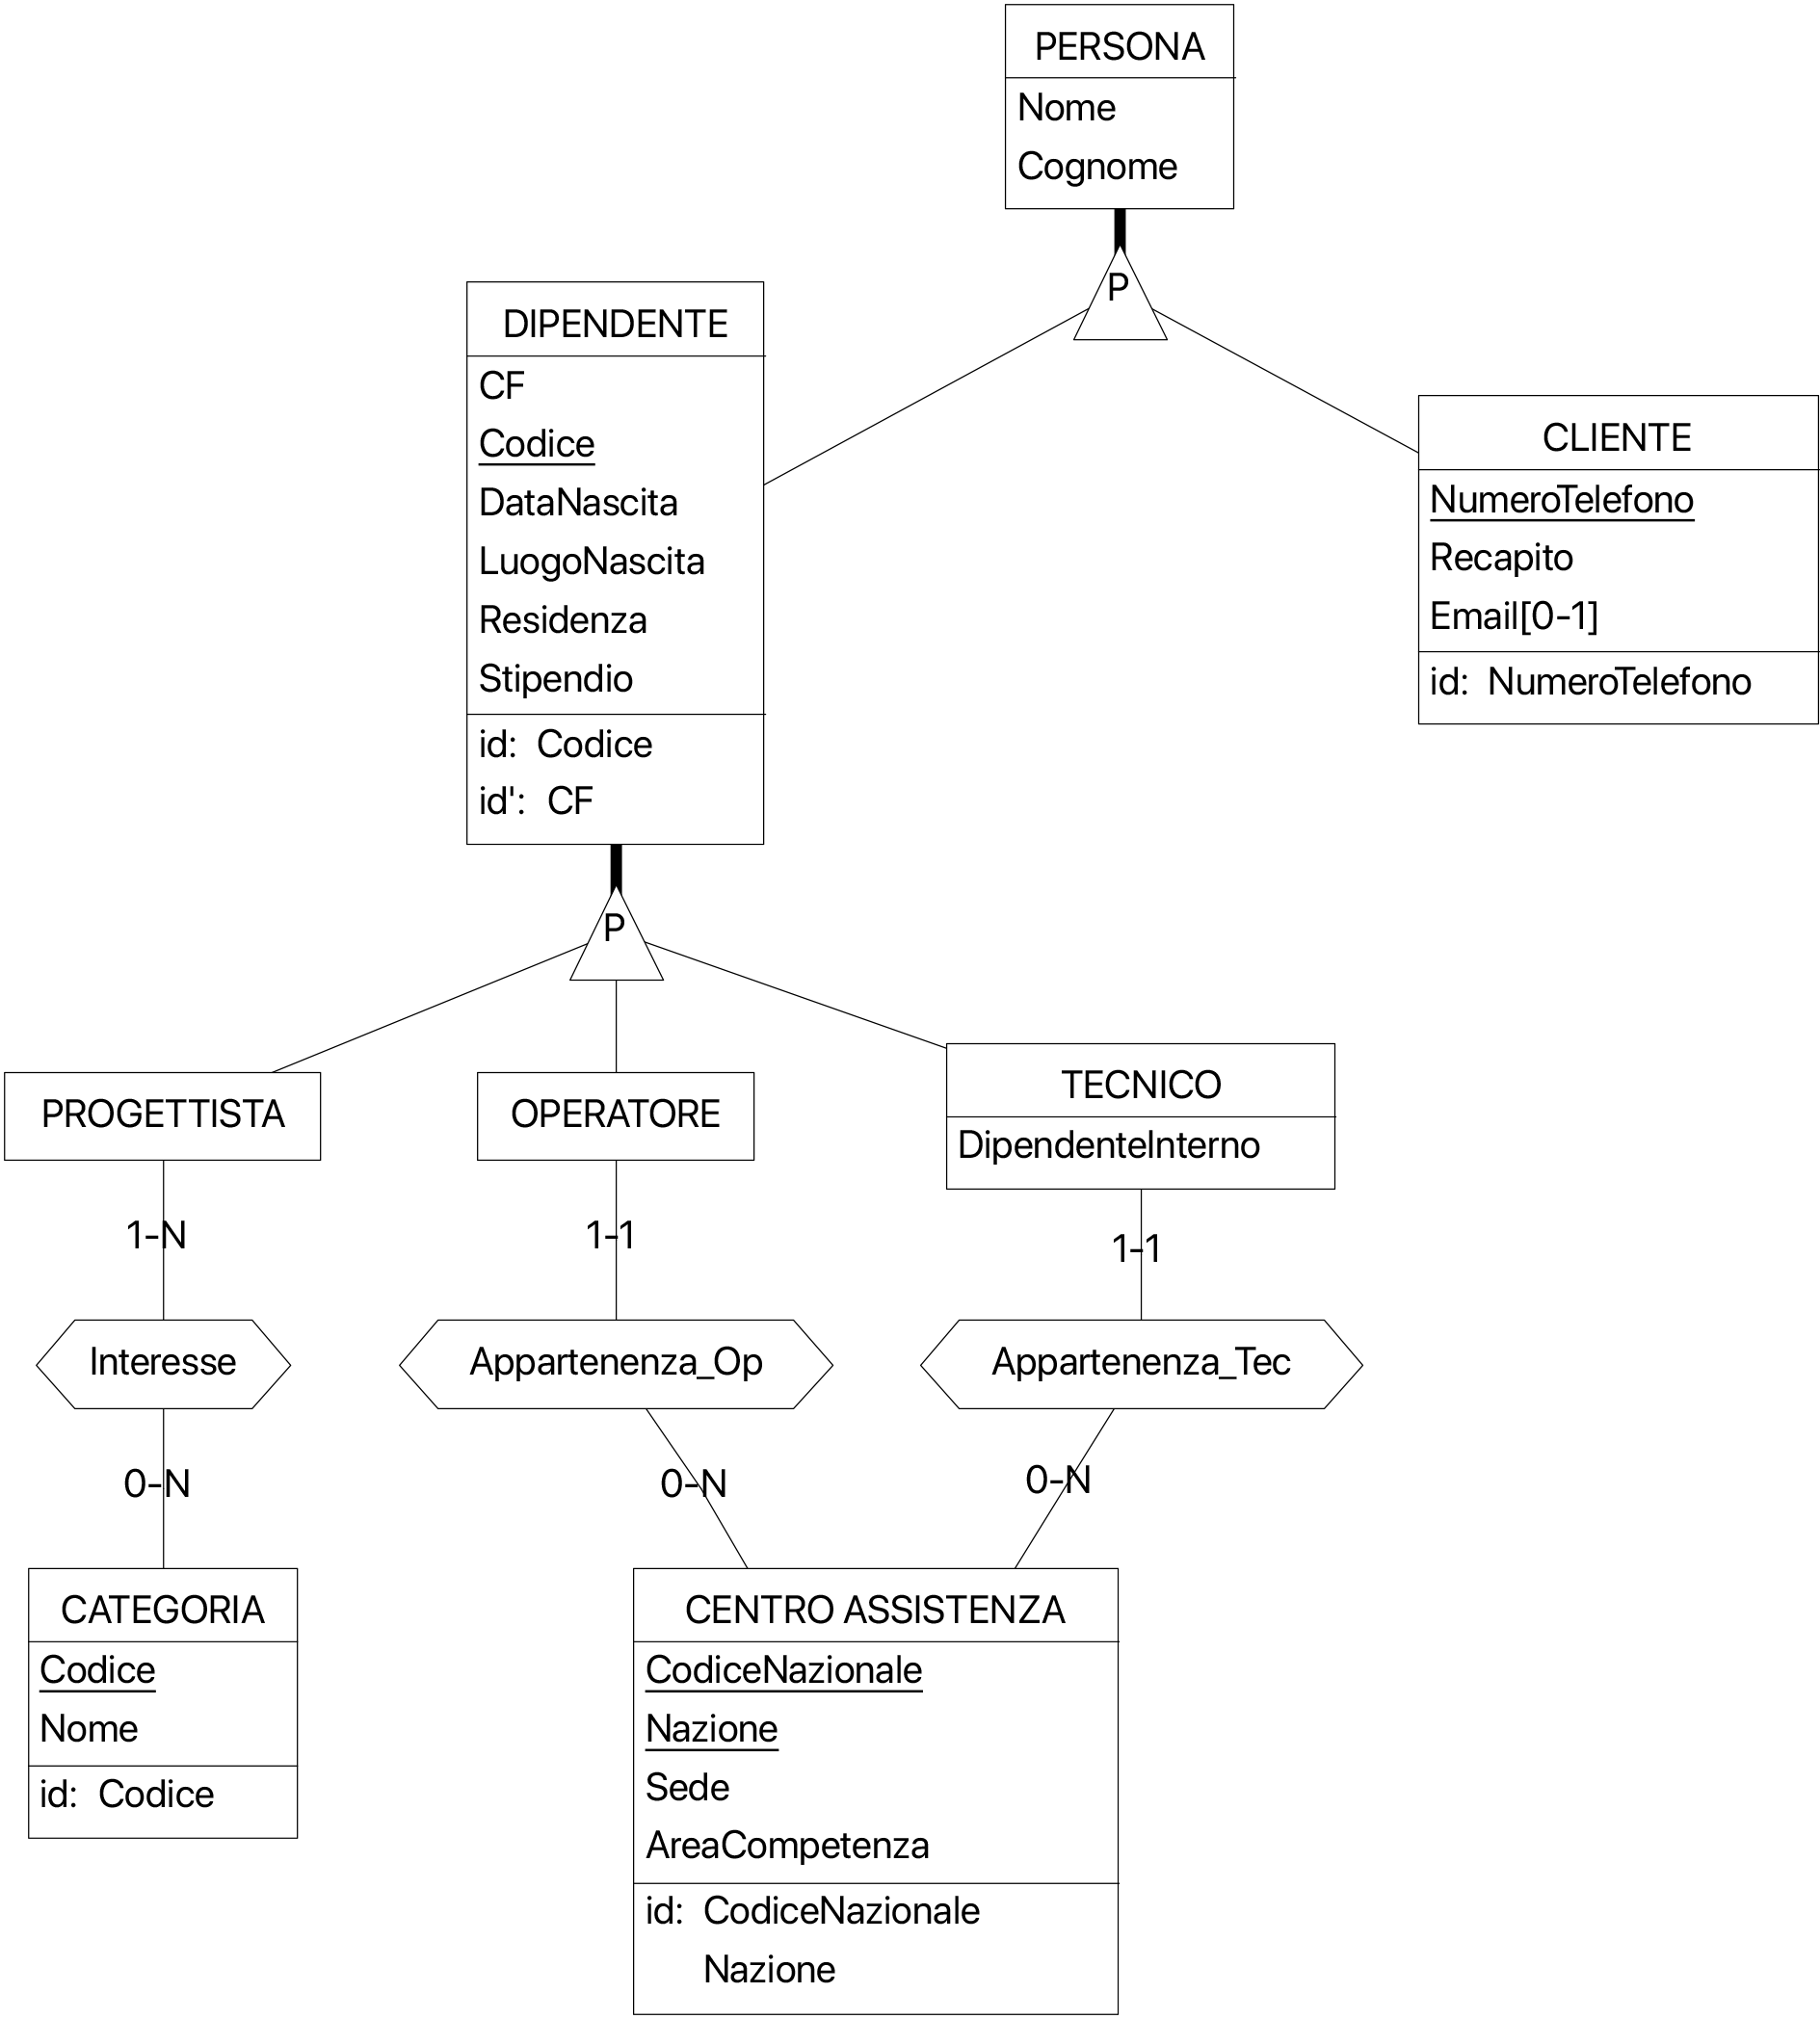
\includegraphics[width=\linewidth]{images/persone.png}
	\caption{Schema raffinato dei concetti riguardanti "persone"}
\end{figure}

\subsection{Centro assistenza}

Il concetto di "centro assistenza", naturale seguito nell'espansione delle specifiche dopo la precedente esplorazione dei concetti legati a persone,
non necessita di molto lavoro per essere sistemato.  

\begin{figure}[H]
	\centering
	\includegraphics[width=\linewidth]{images/centriAssistenza.png}
	\caption{Schema raffinato del concetto "centro assistenza"}
\end{figure}

\subsection{Interventi}

Il cuore delle specifiche è quello che riguarda un "intervento" e i "guasti" che possono accadere ad un prodotto.

\begin{figure}[H]
	\centering
	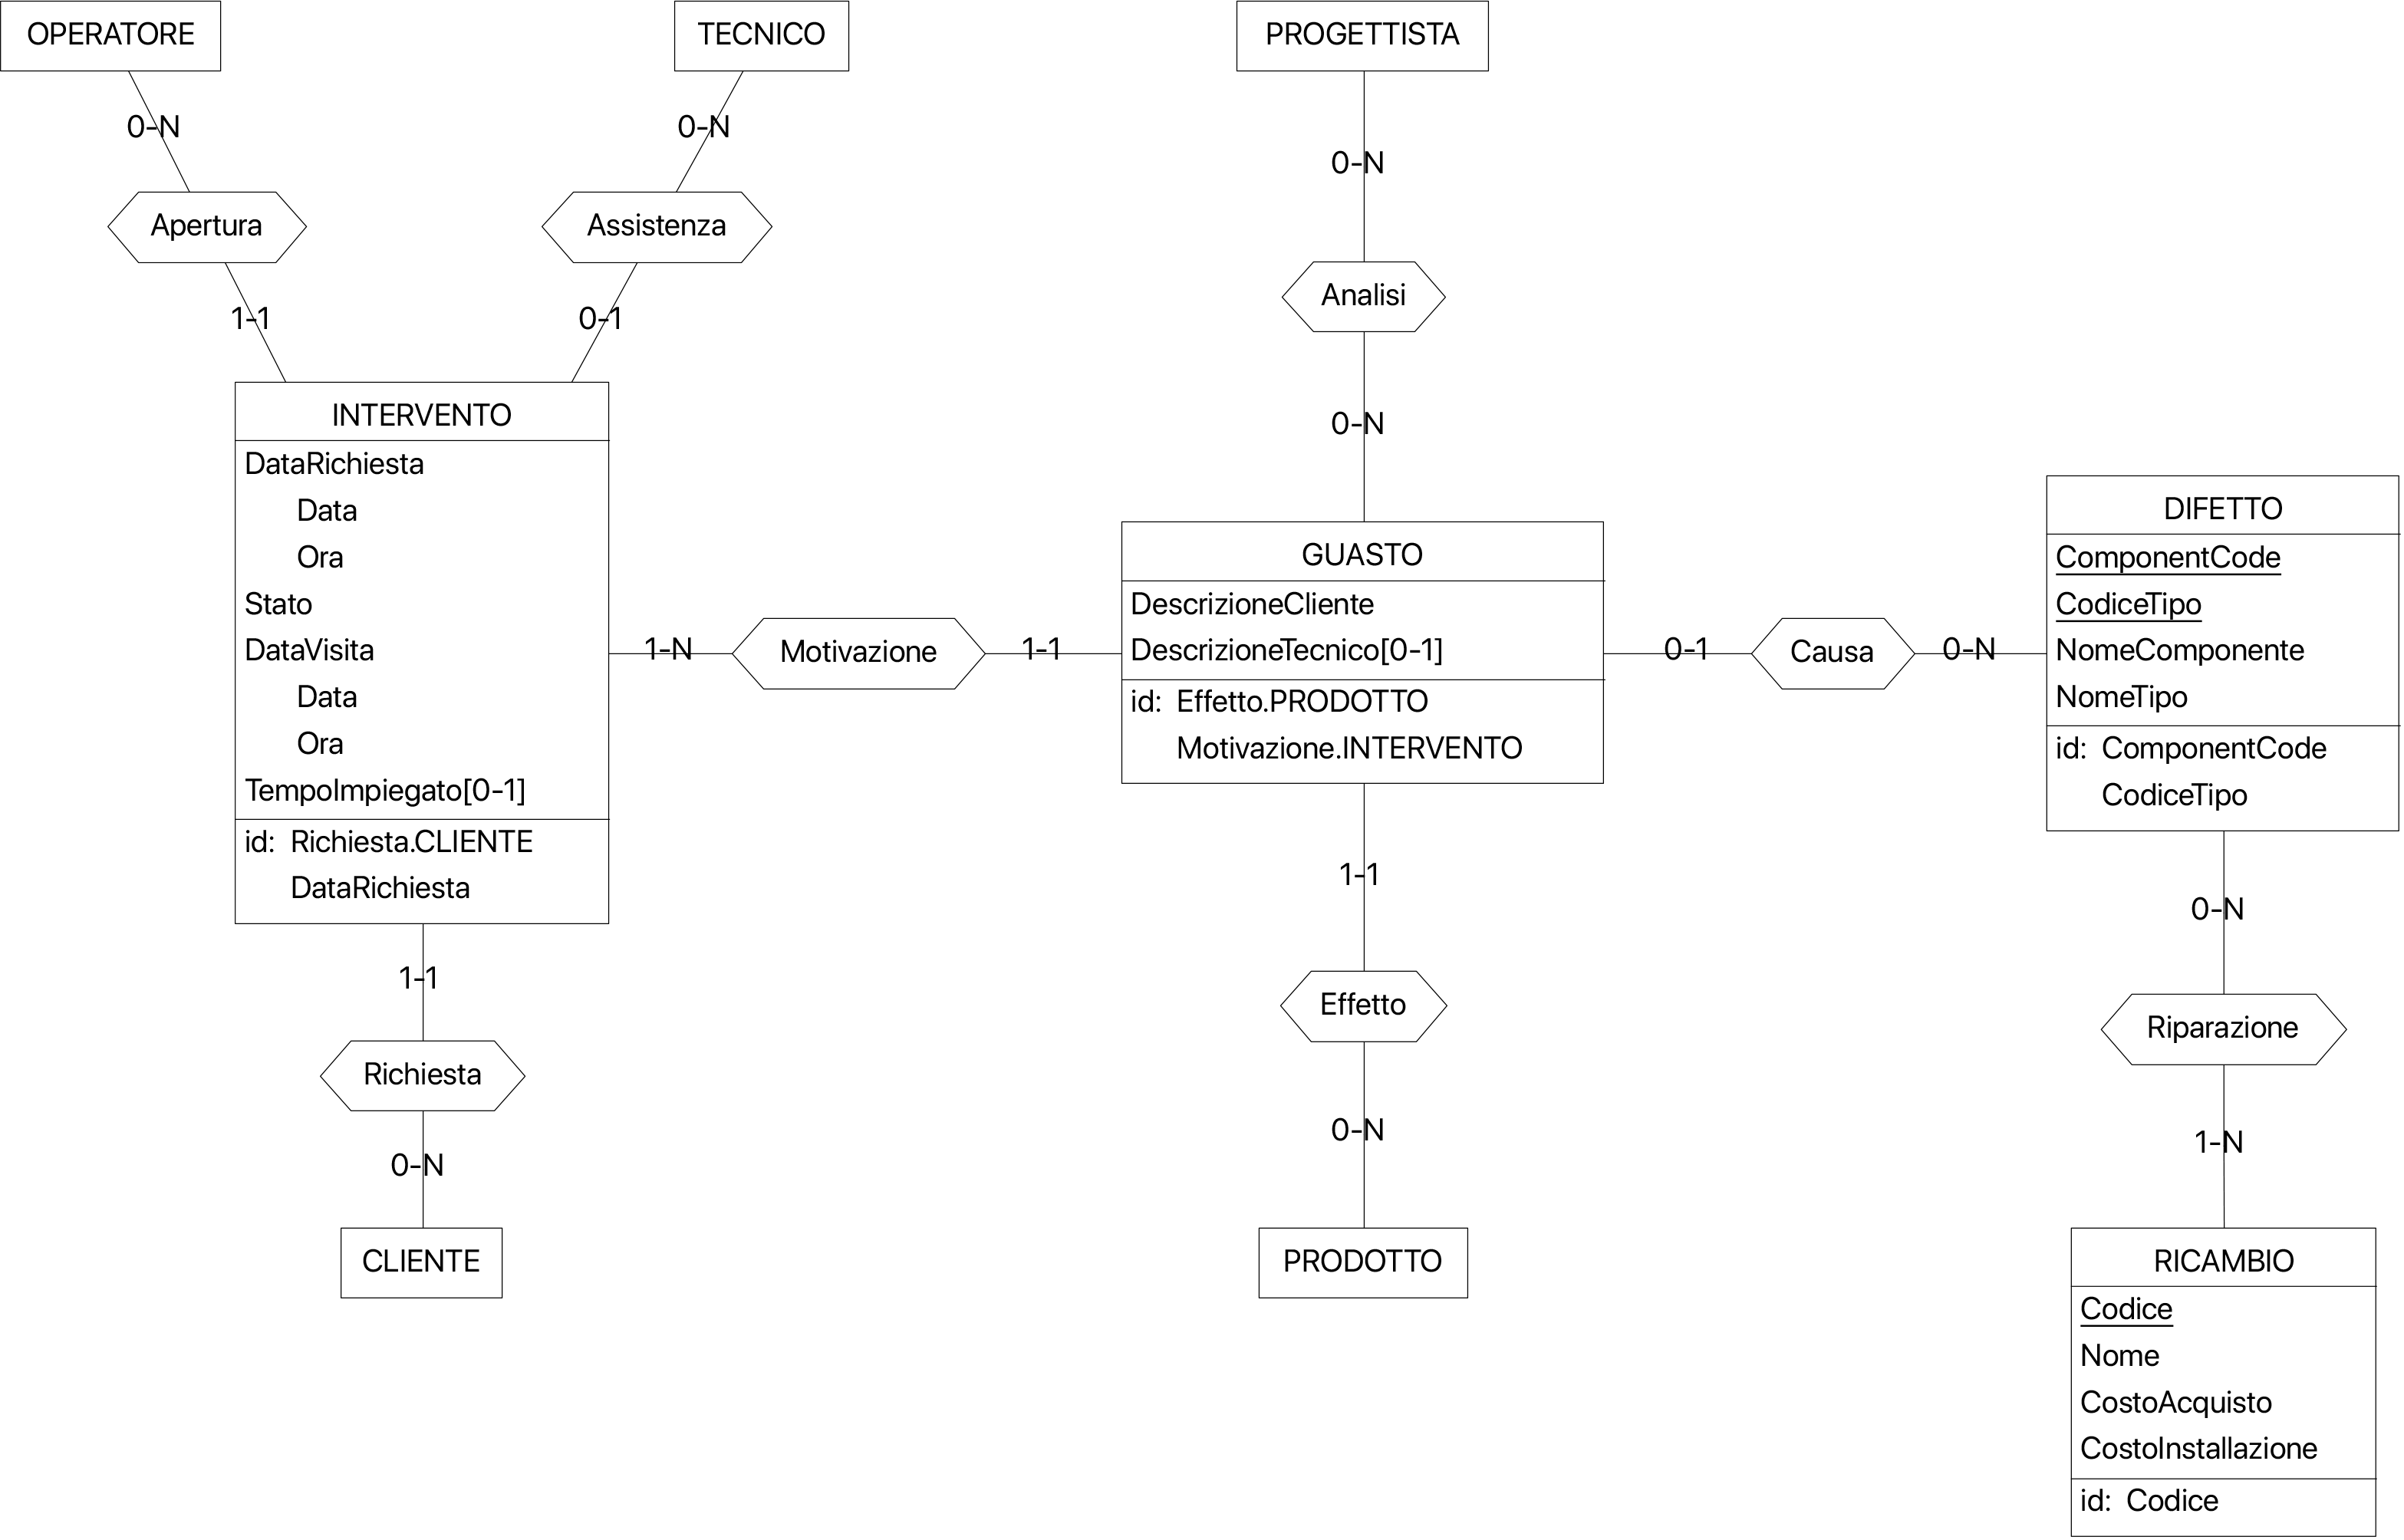
\includegraphics[width=\linewidth]{images/interventi.png}
	\caption{Schema raffinato dei concetti "intervento", "guasto" e "difetto"}
\end{figure}

\subsection{Prodotti}

Da ultimo, espandiamo la nozione di "prodotto".

\begin{figure}[H]
	\centering
	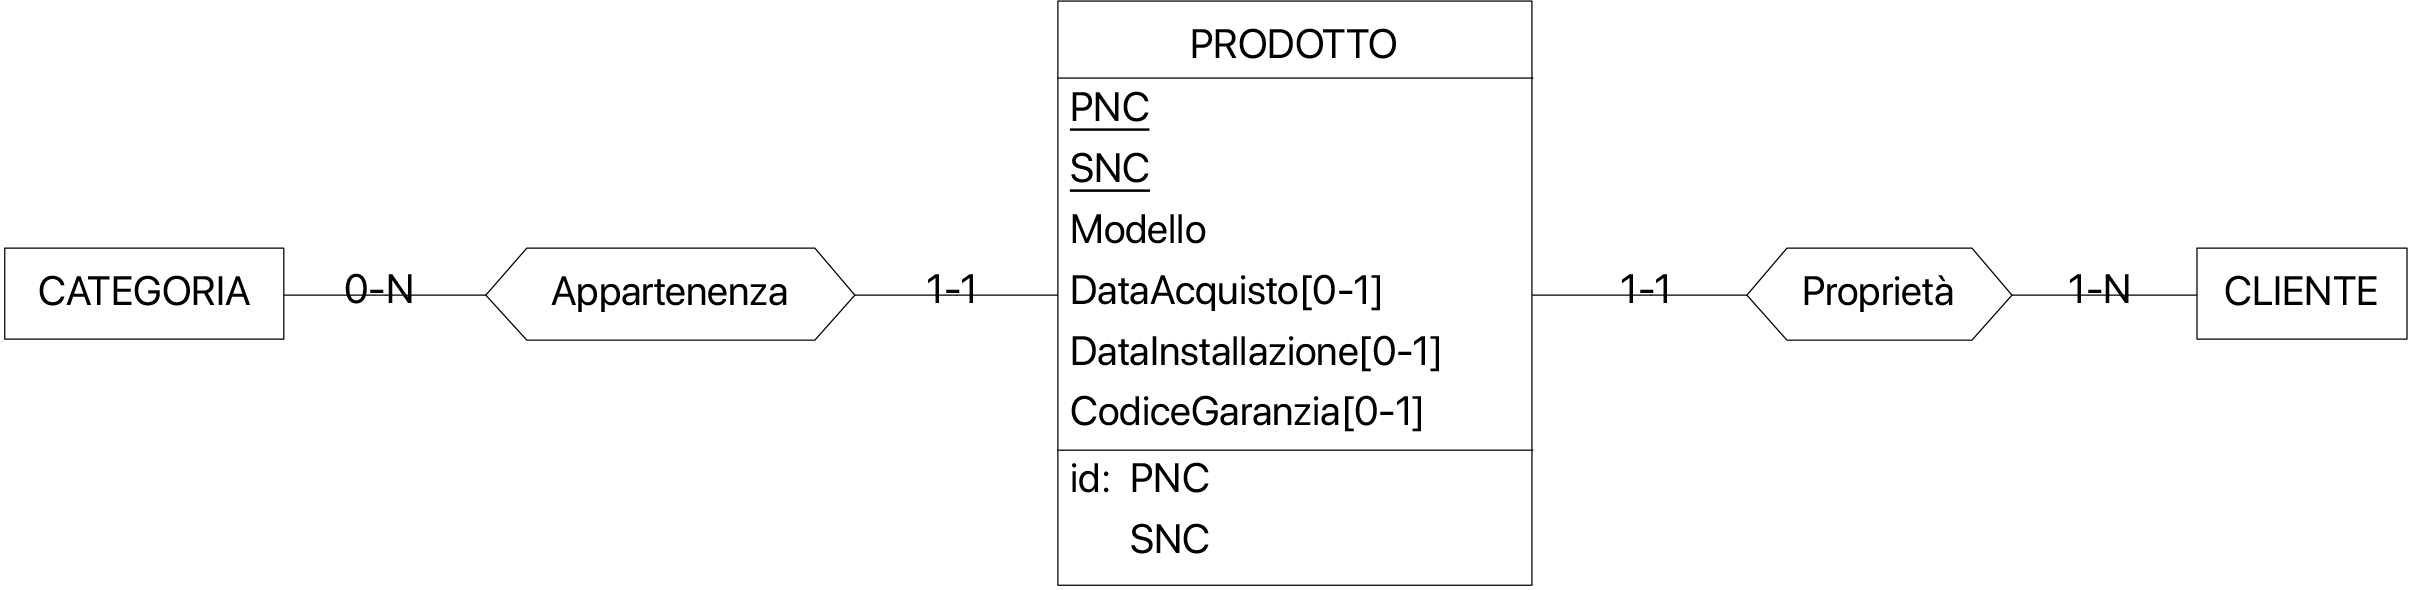
\includegraphics[width=\linewidth]{images/prodotti.png}
	\caption{Schema raffinato del concetto "prodotto" e "modello"}
\end{figure}

\section{Schema finale}

\begin{figure}[H]
	\centering
	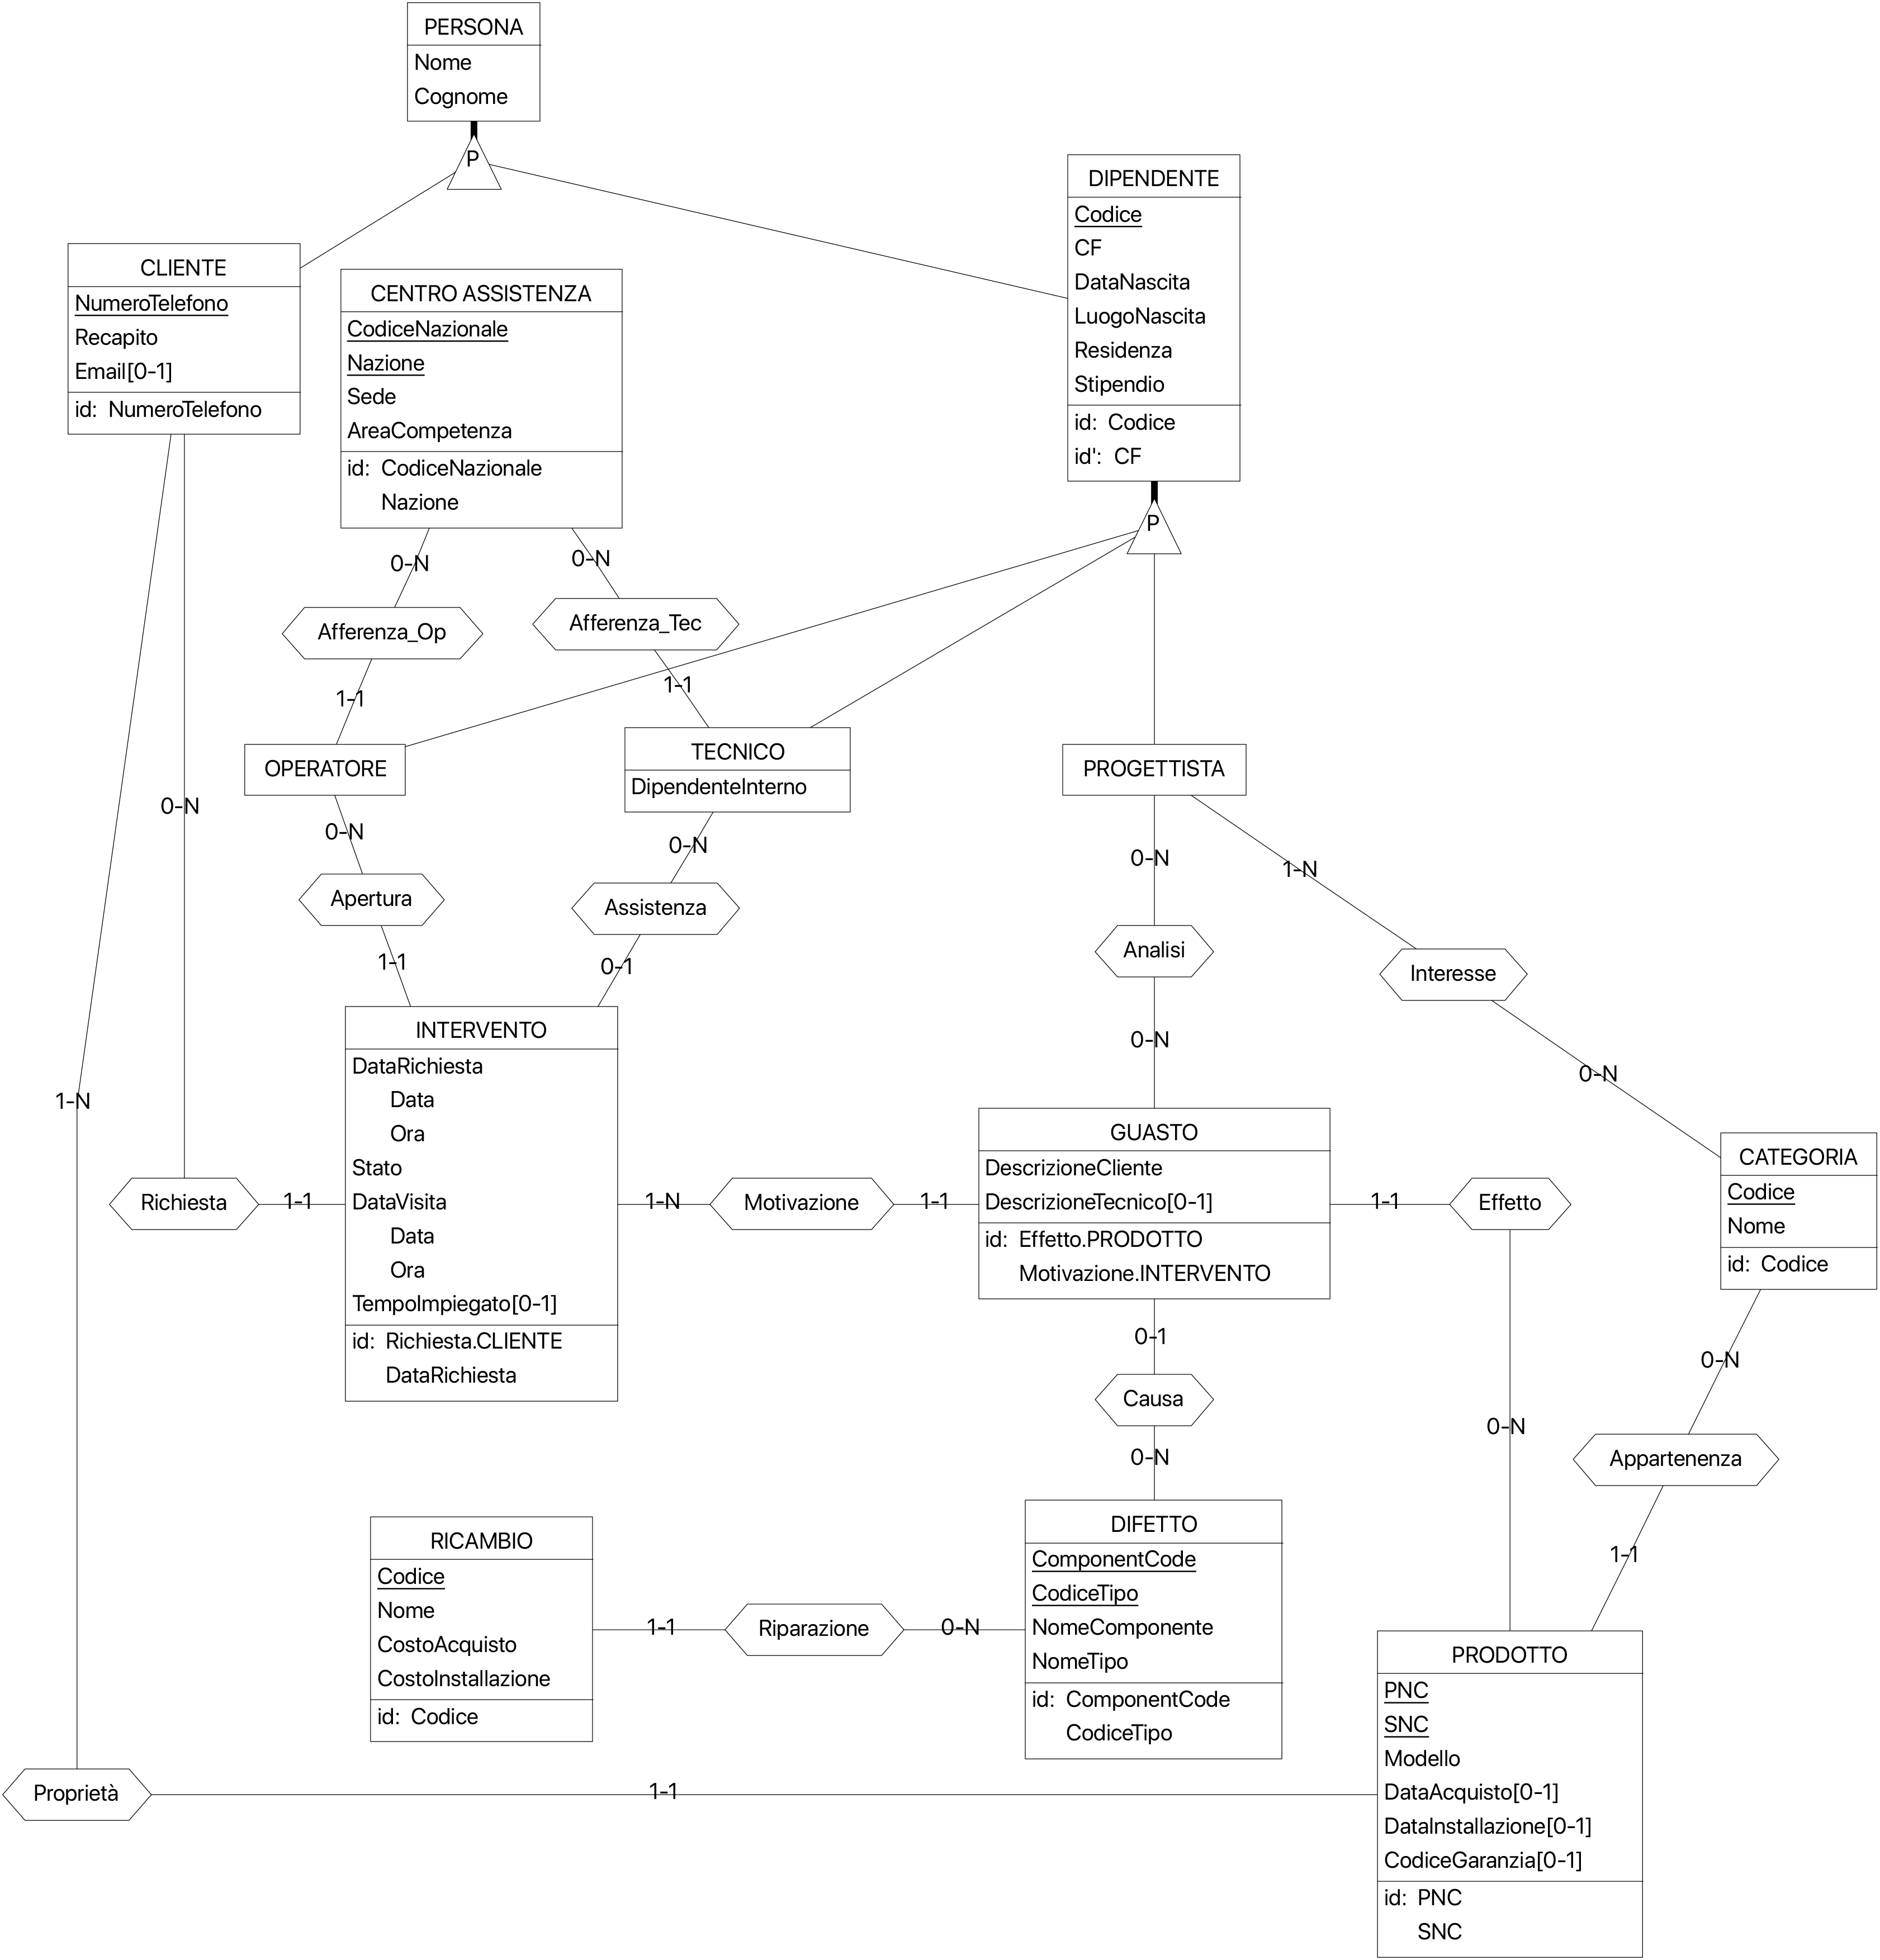
\includegraphics[width=\linewidth]{images/conceptual.png}
	\caption{Schema concettuale finale}
\end{figure}

\chapter{Progettazione logica}

\section{Volume dei dati}

\section{Descrizione e frequenza delle principali operazioni}

\end{document}